\chapter{Interpolation}

\section{Introduction}

\subsection{Definition}

\begin{example}
    Suppose we are given the following population data
    \begin{table}[H]
        \centering
        \begin{tabular}{r|c|c|c|c|c|c|c|c}
            year           & 1940 & 1950 & 1960 & 1970 & 1980 & 1990 & 2000 & 2010 \\
            \hline
            Population (M) & 132  & 151  & 179  & 203  & 226  & 249  & 281  & 308
        \end{tabular}
    \end{table}
    We mey ask the question: what was the population in 1965? We can use \term{interpolation} to estimate the population in 1985.

    \begin{figure}[H]
        \centering
        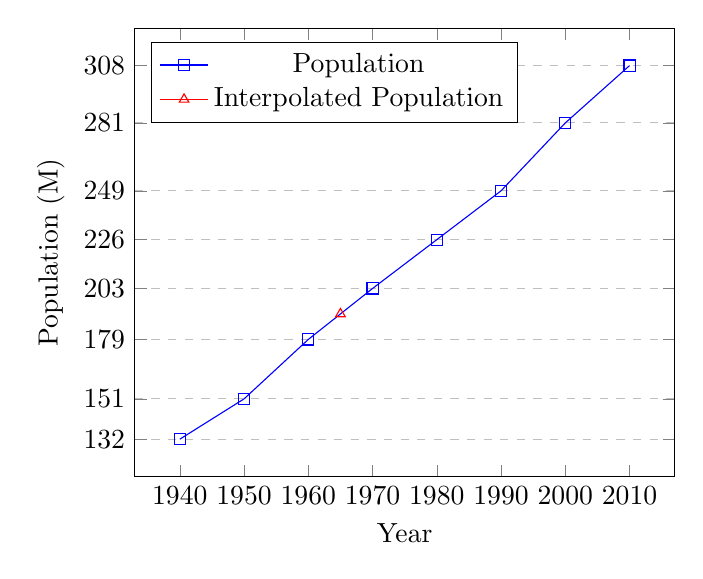
\begin{tikzpicture}
            \begin{axis}[
                    xlabel={Year},
                    ylabel={Population (M)},
                    xtick={1940, 1950, 1960, 1970, 1980, 1990, 2000, 2010},
                    ytick={132, 151, 179, 203, 226, 249, 281, 308},
                    xticklabel style={/pgf/number format/1000 sep=},
                    yticklabel style={/pgf/number format/1000 sep=},
                    legend pos=north west,
                    ymajorgrids=true,
                    grid style=dashed,
                ]

                \addplot[
                    color=blue,
                    mark=square,
                ]
                coordinates {
                        (1940, 132)
                        (1950, 151)
                        (1960, 179)
                        (1970, 203)
                        (1980, 226)
                        (1990, 249)
                        (2000, 281)
                        (2010, 308)
                    };
                \addlegendentry{Population}

                \addplot[
                    color=red,
                    mark=triangle,
                ]
                coordinates {
                        (1965, 191)
                    };
                \addlegendentry{Interpolated Population}

            \end{axis}
        \end{tikzpicture}
        \caption{Population data and interpolated population in 1965}
    \end{figure}

    We may also ask the question: what will the population be in 2020? This will be an \term{extrapolation} problem.
\end{example}

\begin{definition}
    Given a set of \( m \) data points \( \{ (t_i, y_i) \}_{i=1}^{m} \) with \( t_1 < t_2 < \cdots < t_m \), the \textbf{interpolation problem} is to find a function \( g(t) \) from a specific class of functions that \[
        g(t_i) = y_i \quad \text{for all } i = 1, 2, \ldots, m
    \]
\end{definition}

\begin{remark}
    Another use of interpolation is to approximate a function \( f(t) \) by a simpler function \( g(t) \) that is easier to work with.
\end{remark}

\begin{example}
    Suppose we have a function \[
        \operatorname{erf} = \frac{2}{\sqrt{\pi}} \int_{0}^{x} e^{-t^2} \, dt
    \] and we want to approximate it with a polynomial.
    \begin{itemize}
        \item Evaluate \( \operatorname{erf} \) at \( m \) points, \( \{ (x_i, e_i) \}_{i=1}^{m} \)
        \item Interpolate the points with a polynomial \( p(x) \) such that \( p(x_i) = e_i \) for all \( i = 1, 2, \ldots, m \)
        \item Use the interpolant \( p(x) \) in place of \( \operatorname{erf} \)
    \end{itemize}
\end{example}

\subsection{Design Goals for Interpolation}

\begin{enumerate}
    \item Easy to evaluate -- quick, accurate
    \item Gives accurate approximations for \( t \neq t_i \)
    \item Can integrate and differentiate easily
\end{enumerate}

\begin{remark}[Caveats]
    Interpolations come with some caveats.

    \begin{itemize}
        \item Interpolations are not uniques.
        \item Not all interpolations have nice properties
        \item Interpolations does not always give the right solution choice
    \end{itemize}
\end{remark}

\begin{note}
    We assume \textbf{accurate data} has the form \[ \{ (t_i, y_i) \}_{i=1}^m \qquad \text{ or } \qquad \{ t_i, f(t_i) \}_{i=1}^m \] with \[ t_1 < t_2 < \cdots < t_m \]
\end{note}

\subsection{Interpolation Problems}

\begin{example}
    Suppose we want to construct a linear fit for the data \[
        \{ (-1, 2), (1, 1) \}
    \]
    Define \( P_1(t) = b + mt \). We have \( \begin{cases} P_1(-1) = 2 \\ P_1(1) = 1 \end{cases} \implies \begin{cases} b + m (-1) = 2 \\ b + m (1) = 1 \end{cases} \) which yields the solution \[
        b = -\frac{1}{2} \qquad b = \frac{3}{3} \qquad \text{ so } \qquad P_1(t) = \frac{3}{2} - \frac{1}{2}t
    \]
\end{example}

\begin{example}
    Suppose we want to construct a quadratic fit for the data \[
        \{ (-1, 2), (1, 1), (2, 1) \}
    \]
    Define \( P_2(t) = a + bt + ct^2 \). We have \( \begin{cases} P_2(-1) = 2 \\ P_2(1) = 1 \\ P_2(2) = 1 \end{cases} \implies \begin{cases} a + b(-1) + c(-1)^2 = 2 \\ a + b(1) + c(1)^2 = 1 \\ a + b(2) + c(2)^2 = 1 \end{cases} \) which yields \[
        P_2(t) = \frac{4}{3} - \frac{1}{2}t + \frac{1}{6}t^2
    \]
\end{example}

\begin{note}
    We choose polynomial interpolants \[
        P_{m-1}(t) = \sum_{i=1}^m c_i t^{i-1}
    \] because they are easy to evaluate. The operation count is approximately \[
        3n \text{ FLOPs}
    \]
\end{note}

\begin{theorem}[Horner's Rule]
    We can re-write our polynomial as \[
        P_{m-1}(t) = c_1 + t(c_2 + t(c_3 + t(\cdots + t(c_{m-1} + c_m t))))
    \]
\end{theorem}

\begin{note}
    Horner's methods provide some advantages. The operation count reduces to \[
        2m \text{FLOPs}
    \] and it's easier to integrate and differentiate.
\end{note}

\begin{theorem}
    For a set of points \[
        \{ (t_i, y_i) \}_{i=1}^m,
    \] there exists a unique polynomial of degree at less than \( m \) that interpolates the data.
\end{theorem}

\section{Solving Interpolation Problems}

\subsection{Monomial Basis}

Given a set of points \[
    S = \{ (t_i, y_i) \}_{i=1}^m
\] we find the unique polynomial \[
    P_{m-1}(t) = \sum_{i=1}^{m} c_i t^{i-1}
\] that interpolates the data.

Applying the interpolation conditions,
\begin{itemize}
    \item \( P_{m-1}(t_1) = y_1 \)
    \item \( P_{m-1}(t_2) = y_2 \)
    \item \( \vdots \)
    \item \( P_{m-1}(t_m) = y_m \)
\end{itemize}
We have systems of equations
\begin{align*}
    c_1 + c_2 t_1 + c_3 {t_1}^2 + \cdots + c_m {t_1}^{m-1} & = y_1 \\
    c_1 + c_2 t_2 + c_3 {t_2}^2 + \cdots + c_m {t_2}^{m-1} & = y_2 \\
    \vdots                                                         \\
    c_1 + c_2 t_m + c_3 {t_m}^2 + \cdots + c_m {t_m}^{m-1} & = y_m
\end{align*}
That is, a linear system \[
    \begin{pmatrix}
        1      & t_1    & t_1^2  & \cdots & {t_1}^{m-1} \\
        1      & t_2    & t_2^2  & \cdots & {t_2}^{m-1} \\
        \vdots & \vdots & \vdots & \ddots & \vdots      \\
        1      & t_m    & t_m^2  & \cdots & {t_m}^{m-1}
    \end{pmatrix} \begin{pmatrix}
        c_1    \\
        c_2    \\
        \vdots \\
        c_m
    \end{pmatrix} = \begin{pmatrix}
        y_1    \\
        y_2    \\
        \vdots \\
        y_m
    \end{pmatrix}
\]

The matrix \( V \) is called the \term{Vandermonde matrix}.

\begin{lemma}
    If all the \( t_i \) are distinct, then the Vandermonde matrix is invertible.
\end{lemma}

Therefore, we can determine the poly coefficients \( \vec{c} \).

\begin{minted}{python}
    import numpy as np

    t = np.linspace(1.0, 2.0, 11)
    # t = (1.0, 1.1, 1.2, ..., 2.0)

    V = np.vander(t, increasing=True)
    # V = [[1.0, 1.0, 1.0, ..., 1.0],
    #      [1.0, 1.1, 1.21, ..., 2.0],
    #      ...
    #      [1.0, 2.0, 4.0, ..., 1024.0]]

    np.linalg.cond(V)
    # 6518493762298.583 ~ 6.52 * 10^12
\end{minted}

Using IEEE double precision, solving \( V \vec{c} = \vec{y} \) get \( \vec{c}'s \) to approximately 4 significant digits of accuracy. It is difficult to determine interpolants accurately this way.

Originally, we are trying to find \( P_{m-1}(t) \in \P_{m-1} \), write \[
    P_{m-1}(t) = \sum_{i=1}^{m} c_i t^{i-1}
\] using monomial basis \[
    \{ 1, t, t^2, \ldots, t^{m-1} \}
\]

\subsection{Lagrange Basis}

\subsubsection{Using a Different Basis}
Suppose \( \{ b_i(t) \}_{i=1}^{m} \) is a basis for \( \P_{m-1} \), then \[
    P_{m-1}(t) = \sum_{i=1}^{m} \alpha_i b_i(t)
\] for some \( \alpha_i \in \R \) to be determined.

We know that \[
    P_{m-1}(t_i) = y_i
\] and using the new basis, we have
\begin{align*}
    \alpha_1 b_1(t_1) + \alpha_2 b_2(t_1) + \cdots + \alpha_m b_m(t_1)
     & = y_1  \\
    \alpha_1 b_1(t_2) + \alpha_2 b_2(t_2) + \cdots + \alpha_m b_m(t_2)
     & = y_2  \\
     & \vdots \\
    \alpha_1 b_1(t_m) + \alpha_2 b_2(t_m) + \cdots + \alpha_m b_m(t_m)
     & = y_m
\end{align*} which yields the system of equations \[
    \begin{pmatrix}
        b_1(t_1) & b_2(t_1) & \cdots & b_m(t_1) \\
        b_1(t_2) & b_2(t_2) & \cdots & b_m(t_2) \\
        \vdots   & \vdots   & \ddots & \vdots   \\
        b_1(t_m) & b_2(t_m) & \cdots & b_m(t_m)
    \end{pmatrix} \begin{pmatrix}
        \alpha_1 \\
        \alpha_2 \\
        \vdots   \\
        \alpha_m
    \end{pmatrix} = \begin{pmatrix}
        y_1    \\
        y_2    \\
        \vdots \\
        y_m
    \end{pmatrix}
\]

\begin{remark}
    The choice of basis is important. We want to choose a basis that is easy to work with.
\end{remark}

What if \( B = I \)? Then we \( \kappa_I = 1 \) and \( \vec{\alpha} = \vec{y} \).

We choose a basis such that \[
    b_i(t_j) = \begin{cases}
        1 & \text{if } i = j    \\
        0 & \text{if } i \neq j
    \end{cases}
\]

\begin{example}
    Consider \( R = 1 \), we want
    \begin{itemize}
        \item \( b_1 (t_2) = 0 \)
        \item \( b_1 (t_3) = 0 \)
        \item \( \vdots \)
        \item \( b_1 (t_m) = 0 \)
    \end{itemize}

    So if we were to construct a polynomial satisfying these conditions, we would include the factors \[
        (t - t_2) \qquad (t - t_3) \qquad \cdots \qquad (t - t_m)
    \] which suggests \( b_1(t) \) takes the form \[
        (t - t_2)(t - t_3) \cdots (t - t_m)
    \]

    Note that this is of degree \( m-1 \), and since our basis cannot have degree more than \( m-1 \), we cannot add more factors.

    Now we need to satisfy \( b_1(t_1) = 1 \), so we need to divide by a constant. We can choose \[
        b_1(t) = \frac{(t - t_2)(t - t_3) \cdots (t - t_m)}{(t_1 - t_2)(t_1 - t_3) \cdots (t_1 - t_m)}
    \]
\end{example}

In general, \[
    b_k(t) = \frac{\displaystyle\prod_{j=1, j \neq k}^{m} (t - t_j)}{\displaystyle\prod_{j=1, j \neq k}^{m} (t_k - t_j)}
\]

\begin{lemma}
    The set of functions \[
        \{ {b_k}(t) \}_{k=1}^{m}
    \] are linearly independent and form a basis for \( \P_{m-1} \).
\end{lemma}

This basis is know as the \term{Lagrange basis}.

\begin{definition}[Lagrange Basis]\index{Lagrange Basis}
    The \textbf{Lagrange basis} is a set of functions \[
        \{ l_k(t) \}_{k=1}^{m} \qquad \text{where} \qquad l_k(t) =
        \prod_{j=1, j \neq k}^{m} \frac{t - t_j}{t_k - t_j}
    \]
\end{definition}

\begin{remark}
    The Lagrange basis has the property \[
        l_k(t_j) = \begin{cases}
            1 & \text{if } k = j    \\
            0 & \text{if } k \neq j
        \end{cases}
    \]
\end{remark}

The Lagrange form of the interpolating polynomial is \[
    P_{m-1}(t) = \sum_{k=1}^{m} c_k l_k(t) \qquad\text{ where } \vec{c} = \vec{y}
\]

\begin{example}
    We use the Lagrange basis to compute \( P_2(t) \) that interpolates \[
        \{ (-1, 2), (1, 1), (2, 1) \}
    \]

    We have the expressions for the Lagrange basis

    \begin{minipage}[t]{0.3\linewidth}
        \begin{align*}
            l_1(t)
             & = \prod_{k=2,3} \frac{t - t_k}{t_1 - t_k}
            \\
             & = \frac{t - 1}{-1 - 1} \cdot \frac{t - 2}{-1 - 2}
            \\
             & = \frac{1}{6} (t - 1)(t - 2)
        \end{align*}
    \end{minipage}
    \begin{minipage}[t]{0.3\linewidth}
        \begin{align*}
            l_2(t)
             & = \prod_{k=1,3} \frac{t - t_k}{t_2 - t_k}
            \\
             & = \frac{t + 1}{1 + 1} \cdot \frac{t - 2}{1 - 2}
            \\
             & = -\frac{1}{2} (t + 1)(t - 2)
        \end{align*}
    \end{minipage}
    \begin{minipage}[t]{0.3\linewidth}
        \begin{align*}
            l_3(t)
             & = \prod_{k=1,2} \frac{t - t_k}{t_3 - t_k}
            \\
             & = \frac{t + 1}{2 + 1} \cdot \frac{t - 1}{2 - 1}
            \\
             & = \frac{1}{3} (t + 1)(t - 1)
        \end{align*}
    \end{minipage}

    so \begin{align*}
        P_2(t)
         & = 2l_1(t) + 1l_2(t) + 1l_3(t)
        \\
         & = 2 \cdot \frac{1}{6} (t - 1)(t - 2) - \frac{1}{2} (t + 1)(t - 2) + \frac{1}{3} (t + 1)(t - 1)
        \\
         & = \frac{4}{3} - \frac{1}{2}t + \frac{1}{6}t^2
    \end{align*}
    which is the same as the polynomial we found earlier.
\end{example}

\begin{remark}[Lagrange Basis are Expensive]
    For each \( l_i(t) \), we require approximately \( 4m \) FLOPs.
    \begin{itemize}
        \item For the numerator, \( m - 1 \) multiplications and \( m - 1 \) subtractions
        \item For the denominator, \( m - 1 \) multiplications and \( m - 1 \) subtractions
        \item A finial division
    \end{itemize} so we require a total of \[
        \Theta(m^2) \text{ FLOPs}
    \] in total to compute the Lagrange basis.
\end{remark}

\subsection{Newton Basis}

Recall for a general basis \( \{ b_i(t) \}_{i=1}^{m} \), we have \[
    P_{m-1}(t) = \sum_{i=1}^{m} \alpha_i b_i(t)
\] and the interpolating conditions \[
    P_{m-1}(t_i) = y_i
\] We solve the system of equations \[
    B\vec{c} = \vec{y}
\] for \( \vec{c} \), where \[
    B = \begin{pmatrix}
        b_1(t_1) & b_2(t_1) & \cdots & b_m(t_1) \\
        b_1(t_2) & b_2(t_2) & \cdots & b_m(t_2) \\
        \vdots   & \vdots   & \ddots & \vdots   \\
        b_1(t_m) & b_2(t_m) & \cdots & b_m(t_m)
    \end{pmatrix}
\]

We want a \( B \) that is easy to solve, but perhaps not as easy as the identity matrix. We explore a triangular system.

\subsubsection{Lower Triangular System}

We choose a basis \( \{ b_i(t) \}_{i=1}^{m} \) such that \[
    B = \begin{pmatrix}
        b_1(t_1)     & 0            & 0      & \cdots           & 0        \\
        b_1(t_2)     & b_2(t_2)     & 0      & \cdots           & 0        \\
        \vdots       & \vdots       & \ddots & \ddots           & \vdots   \\
        b_1(t_{m-1}) & b_2(t_{m-1}) & \cdots & b_{m-1}(t_{m-1}) & 0        \\
        b_1(t_m)     & b_2(t_m)     & \cdots & b_{m-1}(t_m)     & b_m(t_m)
    \end{pmatrix}
\]

For simplicity, take \( b_1(t) = 1 \).
\begin{itemize}
    \item Row 1: \( b_2(t_1) = 0, b_3(t_1) = 0, \ldots, b_m(t_1) = 0 \)

          We include \( (t - t_1) \) as a factor of each \( b_R(t) \) for \( R = 2, 3, \ldots, m \).

    \item Row 2: \( b_3(t_2) = 0, b_4(t_2) = 0, \ldots, b_m(t_2) = 0 \)

          We include \( (t - t_2) \) as a factor of each \( b_R(t) \) for \( R = 3, 4, \ldots, m \).

    \item \( \vdots \)

    \item Row \( m-1 \): \( b_m(t_{m-1}) = 0 \)

          We include \( (t - t_{m-1}) \) as a factor of \( b_m(t) \).
\end{itemize} which suggests \[
    b_k(t) = \prod_{j=1}^{k-1} (t - t_j)
\]

\begin{remark}
    This is a basis because we have \( m \) linearly independent functions.
\end{remark}

\begin{definition}[Newton Basis]\index{Newton Basis}
    The \term{Newton basis} is a set of functions \[
        \{ n_k(t) \}_{k=1}^{m} \qquad \text{where} \qquad n_k(t) = \prod_{j=1}^{k-1} (t - t_j)
    \]
\end{definition}

The Newton form of the interpolating polynomial is \[
    P_{m-1}(t) = \sum_{k=1}^{m} c_k \prod_{j=1}^{k-1} (t - t_j)
\]

\begin{remark}[Newton Basis are Cheaper]
    If we can remember the results \( t - t_i \), then each new term added would only require \( 3 \) FLOPs. This is a significant improvement over the Lagrange basis. The total operation count is \(
    \Theta(3m) \text{ FLOPs}
    \)
\end{remark}

Now, to determine the coefficients, we solve a lower triangular system \( B\vec{c} = \vec{y} \)
We know that
\begin{itemize}
    \item \( y_1 = P_{m-1}(t_1) = c_1 \) so \[
              c_1 = y_1
          \]
    \item \( y_2 = P_{m-1}(t_2) = c_1 + c_2(t_2 - t_1) \) so \[
              c_2 = \frac{y_2 - c_1}{t_2 - t_1}
          \]
    \item \( \vdots \)
    \item \( \displaystyle y_m = P_{m-1}(t_m) = \sum_{k=1}^{m} c_k \prod_{j=1}^{k-1} (t_m - t_j) \) so \[
              c_m = \frac{\displaystyle y_m - \sum_{j=1}^{m-1} c_j \prod_{k=1}^{j-1} (t_m - t_k)}{\displaystyle \prod_{k=1}^{m-1} (t_m - t_k)}
          \]
\end{itemize}

\begin{example}
    Determine the Newton form of the degree 2 polynomial that interpolates \[
        \{ (-1, 2), (1, 1), (2, 1) \}
    \]

    We have the expressions for the Newton basis
    \begin{itemize}
        \item \( c_1 = y_1 = 2 \)
        \item \( \begin{aligned}[t]
                  c_2 & = \frac{y_2 - c_1}{t_2 - t_1} \\
                      & = \frac{1 - 2}{1 - (-1)}      \\
                      & = -\frac{1}{2}
              \end{aligned} \)
        \item \( \begin{aligned}[t]
                  c_3
                   & = \frac{y_3 - \left[ c_1 + c_2(t_3 - t_1) \right]}{(t_3 - t_1)(t_3 - t_2)}
                  \\
                   & = \frac{1 - \left[ 2 - \frac{1}{2}(2 - (-1)) \right]}{(2 - (-1))(2 - 1)}
                  \\
                   & = \frac{1}{6}
              \end{aligned} \)
    \end{itemize}

    So the Newton form of the interpolating polynomial is \[
        P_2(t) = 2 - \frac{1}{2}(t + 1) + \frac{1}{6}(t + 1)(t - 1) = \frac{4}{3} - \frac{1}{2}t + \frac{1}{6}t^2
    \]

    This is the same polynomial we found earlier with the monomial and Lagrange basis.
\end{example}

\subsection{Summary}

% \begin{table}[H]
%     \centering
%     \begin{tabular}{r|c|c|c|c}
%          & \small Evaluate \( P_{m-1}(t) \)
%          & \small Integrate/Differentiate
%          & \small Finding Coefficients
%          & \small Add \( (t_{m+1}, g_{m_1}) \)
%         \\ \hline
%         \small Monomial Basis
%          & \small Easy
%          & \small Easy
%          & \small Can be Ill-conditioned
%          & \small All Coefficients Change
%         \\
%         \small Lagrange Basis
%          & \small Difficult
%          & \small Difficult
%          & \small Very Easy
%          & \small Just add \( \frac{t - t_{m+1}}{t - t_m} \) to each \( l_k(t) \)
%         \\
%         \small Newton Basis
%          & \small Easy
%          & \small Medium
%          & \small Easy
%          & \small Add \( c_m \cdot ( t - t_1) \cdot \ldots \cdot (t - t_{m-1}) \) to previous interpolants
%     \end{tabular}
% \end{table}

\begin{table}[H]
    \centering
    \begin{tabular}{r|p{3.5cm}|p{3.5cm}|p{4cm}}
         & \small \bold{Monomial Basis}
         & \small \bold{Lagrange Basis}
         & \small \bold{Newton Basis}
        \\ \hline
        \small Evaluate \( P_{m-1}(t) \)
         & \small Easy
         & \small Difficult
         & \small Easy
        \\ \hline
        \small Integrate/Differentiate
         & \small Easy
         & \small Difficult
         & \small Medium
        \\ \hline
        \small Finding Coefficients
         & \small Can be Ill-conditioned
         & \small Very Easy
         & \small Easy
        \\ \hline
        \small Add \( (t_{m+1}, g_{m+1}) \)
         & \small All Coefficients Change
         & \small Just add \( \frac{t - t_{m+1}}{t - t_m} \) to each \( l_k(t) \)
         & \small Add \( \displaystyle c_m \prod_{j=1}^{m-1} (t - t_j) \) to previous interpolants
    \end{tabular}
\end{table}

\section{Error Analysis}

What about accuracy? We know \[
    P_{m-1}(t_i) = y_i \quad \text{for all } i = 1, 2, \ldots, m
\] but how can we determine if \( P_{m-1}(t) \) is a good approximation for \( f(t) \) for \( t \neq t_i \)?

\begin{theorem}
    Suppose the polynomial \( P_{m-1}(t) \) interpolates the function \( f(t) \) at distinct points \( t_1 < t_2 < \cdots < t_m \). If \( f \) is \(m\)-times differentiable on the interval \([t_1, t_m]\), then for any point \( t \in [t_1, t_m] \), \[
        f(t) - p_{m-1}(t) = \frac{1}{m!} f^{(m)}(c_t) \omega_m(t)
    \] where
    \begin{itemize}
        \item \( c_t \) is some point in \( t_1, t_, \) that depends on \( t \);
        \item \( \displaystyle \omega_m(t) = (t - t_1) (t - t_2) \cdots (t - t_m) = \prod_{j=1}^{m} (t - t_j) \)
    \end{itemize}
\end{theorem}

We have \[
    \max_{t \in [t_1, t_m]} | f(t) - P_{m-1}(t) | \leq \frac{1}{m!} \max_{t \in [t_1, t_m]} | f^{(m)}(t) | \max_{t \in [t_1, t_m]} | \omega_m(t) |
\]
\begin{itemize}
    \item \( m \) is the interpolation points we can control
    \item \( f^{(m)}(t) \) is the \( m \)-th derivative of \( f(t) \) which is the function we are trying to approximate
    \item depends on placement of \( t_i \) in the interval \([t_1, t_m]\)
    \item We can show that \[
              \max_{t \in [t_1, t_m]} | \omega_m(t) | \leq \frac{h^m \cdot (m - 1)!}{4}
          \] where \[
              h = \max_{i = 1, \dots, m-1} | t_{i+1} - t_i |
          \]
\end{itemize}

Thus, \begin{align*}
    \max_{t \in [t_1, t_m]} | f(t) - P_{m-1}(t) |
     & \leq \frac{1}{m!} \max_{t \in [t_1, t_m]} | f^{(m)}(t) | \frac{h^m \cdot (m - 1)!}{4}
    \\
     & \leq \frac{M \cdot h^m}{4m}
\end{align*} where \[
    M = \max_{t \in [t_1, t_m]} | f^{(m)}(t) |
\]

If we add mode interpolation points (increasing \( m \)), while keeping \( t_m - t_1 \) fixed, will the error do down?

We know that \[
    \text{error} \leq \frac{1}{4m} \cdot M \cdot h^m
\] and as we increase \( m \),
\begin{itemize}
    \item \( \frac{1}{4m} \) decreases
    \item The behaviour of \( h^m \) depends on yhe function
    \item \( h^m \) decreases for \( h < 1 \)
\end{itemize}

\begin{example}
    Consider \[
        f(t) = \sin(\pi t)
    \] and we interpolate at equally spaced points on \( [-1, 1] \).

    \begin{itemize}
        \item For \( m = 4 \), \( t_i \in \{ -1, -\sfrac{1}{3}, \sfrac{1}{3}, 1 \} \), and the interpolant is \( P_3(t) \).
        \item For \( m = 7 \), \( t_i \in \{ -1, -\sfrac{2}{3}, -\sfrac{1}{3}, 0, \sfrac{1}{3}, \sfrac{2}{3}, 1 \} \), and the interpolant is \( P_6(t) \).
        \item For \( m = 10 \), \( t_i \in \{ -1, -\sfrac{7}{9}, \dots, \sfrac{7}{9}, 1 \} \), and the interpolant is \( P_9(t) \).
    \end{itemize}

    % TODO: Plot

    We have \[
        \max_{t \in [-1, 1]} | f^{(m)}(t) | = \pi^m
    \]
\end{example}

\begin{example}
    Consider the Rauge's function \[
        f(t) = \frac{1}{1 + 25t^2}
    \] and we interpolate at equally spaced points on \( [-1, 1] \).

    Consider \( m = 4, m = 7, m = 10, \) and \( m = 13 \).

    % TODO: Plot

    We observe that in the middle area, the approximation gets better with increasing \( m \). However, at the ends, the error is bigger and the approximation is less accurate.
\end{example}

\begin{remark}
    Degree \( m - 1 \) polynomial interpolants does not necessarily converge to the function that they interpolate as \( m \) increases.
\end{remark}

\section{Piecewise Polynomial Interpolation}

What should we do if we need to interpolate a large dataset?

\subsection{Piecewise-Linear Interpolation}

The idea is to split the data into smaller chunks and interpolate each chunk separately. We construct \term{piecewise polynomial interpolants} \[
    \{ P_{d,i}(t) \}
\] where
\begin{itemize}
    \item \( d \) is the degree of the polynomial
    \item \( i \) is the interval number
\end{itemize}

\begin{example}[Piecewise-linear]
    Given \( \{ (t_1, y_i ) \}_{i=1}^{m} \), a piecewise-linear interpolant is \[
        \{ P_{1,i}(t) \}_{i=1}^{m-1}
    \]

    We define the interpolant \[
        L(t) = \{ P_{1,i}(t) \text{ where } t \in [t_i, t_{i+1}] \}
    \]

    The \( \{ t_i \}_{i=1}^{m} \) are called the \term{knots} of the piecewise-linear interpolant.

        {~~~}

    \begin{itemize}
        \item If we consider Lagrange polynomials, we have \[
                  P_{1,i}(t) = y_i \frac{t-t_{i+1}}{t_i - t_{i+1}} + y_{i+1} \frac{t-t_i}{t_{i+1} - t_i}
              \]

        \item If we consider Newton polynomials, we have \[
                  P_{1,i}(t) = y_i + \frac{y_{i+1} - y_i}{t_{i+1} - t_i} (t - t_i)
              \]
    \end{itemize}
\end{example}

\begin{remark}
    \( L(t) \) is continuous. Indeed,
    \begin{itemize}
        \item Each piece is linear
        \item Connection at knots \[
                  P_{1,i}(t_{i+1}) = y_{i+1} = P_{1,{i+1}}(t_{i+1})
              \]
    \end{itemize}
\end{remark}

\begin{remark}
    \[
        {P_{1,i}}'(t) = \frac{y_{i+1} - y_i}{t_{i+1} - t_i}
        \qquad
        {P_{1,i+1}}'(t) = \frac{y_{i+2}-y_{i+1}}{t_{i+2}-t_{i+1}}
    \]
\end{remark}

\subsubsection{Accuracy}

Suppose \( L(t) \) interpolates \( f(x) \) at knots \( \{ t_i \}_{i=1}^{m} \).
We have \[
    f(t) - L(t) = f(t) - P_{1,i}(t) = \frac{1}{2!} f''(c_t) \Big[ (t - t_i)(t - t_{i+1}) \Big]
\] for some \[
    c_t \in ( t_i, t_{i+1} )
\]

Note that the second derative stays the same, and \begin{align*}
    \omega_2(t)
     & = (t - t_i)(t - t_{i+1})
    \\
     & = t^2 - (t_i + t_{i+1})t + t_{i}t_{i+1}
\end{align*}

We check the boundaries and the critical points \[
    \omega'(t) = 2t - (t_i+t_{i+1})\omega_2(t_i) = 0
    \qquad \text{and} \qquad
    \omega'(t) = 2t - (t_i+t_{i+1})\omega_2(t_{i+1}) = 0
\]

\( \omega_2 \) is part of a quadratic so the maximum of absolute values happens at the centre \[
    \frac{t_{i} + t_{i+1}}{2}
\]

% TODO: Some stuff there

For \( t \in [t_1, t_m] \), \[
    | L(t) - f(t) | \leq \frac{1}{2!} \cdot \frac{h^2}{4} \cdot \max_{t \in [t_1, t_m]} | f''(t) | = \frac{h^2}{8} \cdot \max_{t \in [t_1, t_m]} | f''(t) |
\] where \( h = \max_{i} h_i \)

For uniformly spaced \( t_i \), increasing the number of interpolation points would reults in smaller \( h \), leading to a lower error.

\subsection{Piecewise-Cubic Interpolation}
% TODO: Plots

We observe that partial-linear interpolations struggles when there is curvature.

Instead, we consider a piece-wise cubic interpolation.

For each \( [t_i, t_{i+1}] \), we fit a cubic \( P_{3,i}(t) \) where \( t \in [t_i, t_{i+1}] \).

On each sub-interval, we need to determine \[
    P_{3,i} = \alpha_i + \beta_i(t - t_i) + \gamma_i(t - t_i)^2 + \delta_i(t - t_i)^3
\]

For \( t = t_i \), we have \[
    P_{3,i}(t_i) = \alpha_i = f(t_i)
\] and for \( t = t_{i+1} \), we have \[
    P_{3,i}(t_{i+1}) = \alpha_i + \beta_i h_i^1 + \gamma_i h_i^2 + \delta_i h_i^3
\] where \( h_i = t_{i+1} - t_i \).

\begin{remark}
    The algorithm requires the derivatives \[
        P_{3,i}'(t) = \beta_i + 2\gamma_i(t - t_i) + 3\delta_i(t - t_i)^2
    \]

    We have \[
        P_{3,i}'(t_i) = \beta_i = f'(t_i)
        \qquad
        P_{3,i}'(t_{i+1}) = \beta_i + 2\gamma_i h_i + 3\delta_i h_i^2 = f'(t_{i+1})
    \]
\end{remark}

We need to solve \[
    \begin{bmatrix}
        1 & 0   & 0     & 0      \\
        0 & 1   & 0     & 0      \\
        1 & h_i & h_i^2 & h_i^3  \\
        0 & 1   & 2h_i  & 3h_i^2
    \end{bmatrix} \begin{bmatrix}
        \alpha_i \\ \beta_i \\ \gamma_i \\ \delta_i
    \end{bmatrix} = \begin{bmatrix}
        f(t_i) \\ f'(t_i) \\ f(t_{i+1}) \\ f'(t_{i+1})
    \end{bmatrix}
\] for each interval \( [t_i, t_{i+1}] \). We get a \term{piecewise cubic Hermite interpolant} (PCHIP)\index{Piecewise Cubic Hermite Interpolant (PCHIP)}.

\begin{remark}[Caveat]
    The PCHIP requires the derivatives of the function. This means that we need to know the function \( f(t) \) in advance.
\end{remark}

What happens if we are only given a set of points, and not the function itself? We construct a \term{cubic spline interpolation}.

\begin{example}
    Suppose \( m = 4 \), and we are given \[
        (t_1, y_1), (t_2, y_2), (t_3, y_3), (t_4, y_4)
    \]

    Define \( S(t) = \{ S_i(t) \text{ if } t \in [t_1, t_{i+1}] \} \)

    Hence we are to determine \[
        S_1(t), S_2(t), S_3(t)
    \]

    Let \( s_i(t) = a_i + b_i(t - t_i) + c_i(t - t_i)^2 + d_i(t - t_i)^3 \) for \( t \in [t_i, t_{i+1}] \).

    There are 4 unknown coefficients per interval -- in general, \( 4(m - 1) \) unknown coefficients to determine.

    \begin{itemize}
        \item What do we know?
              We want \( S(t) \) to interpolate data.

              The left end points
              \begin{itemize}
                  \item \( S_1(t_1) = y_1 \)
                  \item \( S_2(t_2) = y_2 \).
                  \item \( S_3(t_3) = y_3 \).
                  \item \( \vdots \)
                  \item \( S_{m-1}(t_{m-1}) = y_{m-1} \).
              \end{itemize}
              The right end points
              \begin{itemize}
                  \item \( S_1(t_2) = y_2 \)
                  \item \( S_2(t_3) = y_3 \).
                  \item \( S_3(t_4) = y_4 \).
                  \item \( \vdots \)
                  \item \( S_{m-1}(t_m) = y_m \).
              \end{itemize}

        \item We want \( S(t) \) to be smooth.

              \begin{itemize}
                  \item \( S_i(t) \) is differentiable since it is a cubic polynomial.
                  \item The issues happen at the knots \( t_i \).
              \end{itemize}

              We require \[
                  s_i'(t + 1) = s_{i+1}'(t_{i+1}) \qquad \text{for } i = 1, 2, \ldots, m-2
              \] and this proposes \( m - 2 \) more constraints on the coefficients.
    \end{itemize}

    In total, we have \( 4(m - 1) \) unknowns and \[
        2(m-1) + (m-2) + (m-2) = 4m - 6
    \] constraints.

    The second \( m-2 \) comes from the constraints at the second derivatives. We require \[
        S_1''(y_2) = S_2''(t_2) \qquad S_2''(t_3) = S_3''(t_3) \qquad \dots \qquad s_{m-2}''(t_{m-1}) = s_{m-1}''(t_{m-1})
    \]
\end{example}

\begin{remark}
    In SciPy, we could use the \texttt{scipy.interpolate.CubicSpline} function.
\end{remark}

We realize that we are two constraints short. We could further impose constrains on the derivatives at the ends.

\begin{itemize}
    \item \( S_1''(t_1) = 0 \), \( S_{m-1}''(t_m) = 0 \) are called \term{natural spline} boundary conditions.
    \item If \( y' \) are known at the ends, we have \( s_1'(t_1) = y_1' \) and \( s_{m-1}'(t_m) = y_m' \) which are called \term{clamped spline} boundary conditions.
    \item We force \( S_1'''(t_2) = S_2'''(t_2) \) and \( S_{m-2}'''(t_{m-1}) = S_{m-1}'''(t_{m-1}) \) which are called \term{not-a-knot spline} boundary conditions.
\end{itemize}

\subsection{Accuracies of the Cubic Splines}

\begin{theorem}
    Let \( f \in C^4[a, b] \).

    If \( S(t) \) is a natural or clamped or not-a-knot cubic spline that interpolates \( f(t) \) at \( a = t_1 < t_2 < \cdots < t_m = b \), then \[
        \max_{t \in [a, b]} | S(t) - f(t) | \leq C_{\text{method}} \cdot h^4 \cdot \max_{t \in [a, b]} | f^{(4)}(t) |
    \] where
    \begin{itemize}
        \item \( C_{\text{method}} \) is a small constant dependent on the type of spline
              \begin{itemize}
                  \item \( C_{\text{clamped}} = \frac{5}{384} \)
                  \item \( C_{\text{not-a-knot}} = \frac{5}{384} \)
              \end{itemize}
        \item \( h = \max_{i} h_i = \max_{i} t_{i+1}-t_i \) is the maximum distance between knots
    \end{itemize}
\end{theorem}

Suppose uniformally spaced knots, \[
    h = \frac{b - a}{m - 1}
\] If we double the amount of interpolation points, \( h \to h/2 \), and the error goes down by a factor of \( 2^4 = 16 \).

\begin{remark}
    For derivative approximations, \[
        \max_{t \in [a,b]} | f^{(p)}(t) - S^{(p)}(t) | \leq C_{\text{method}} \cdot h^{4-p} \cdot \max_{t \in [a, b]} | f^{(4)}(t) |
    \] for \( p = 0, 1, 2 \).
\end{remark}

\subsection{Calculating Cubic Spline}

Given the set of points \( \{ (t_i, y_i) \}_{i=1}^{m} \), we want to determine the coefficients of the cubic spline \[
    S(t) = \{ s_i(t) \text{ when } t \in [t_i, t_{i+1}] \}
\]

Take \[
    S_i(t) = a_i + b_i(t - t_i) + c_i(t - t_i)^2 + d_i(t - t_i)^3
\] for \( i = 1 \) to \( m - 1 \).

\begin{itemize}
    \item \( S'(t) = b_i + 2c_i(t - t_i) + 3d_i(t - t_i)^2 \)
    \item \( S''(t) = 2c_i + 6d_i(t - t_i) \)
    \item \( S'''(t) = 6d_i \)
\end{itemize}

We want \( S(t) \) to be a continuous interpolant.
\begin{equation}\label{eq:cubic-spline-1}
    S_i(t_i) = y_i \qquad \text{ for } i = 1 \text{ to } m-1
\end{equation}\begin{equation}\label{eq:cubic-spline-2}
    S_i(t_{i+1}) = y_{i+1} \qquad \text{ for } i = 1 \text{ to } m-1
\end{equation}

For \( S \) to have 2 continuous derivatives, we require \begin{equation}\label{eq:cubic-spline-3}
    S_i'(t_{i+1}) = S_{i+1}'(t_{i+1}) \qquad \text{ for } i = 1 \text{ to } m-2
\end{equation}\begin{equation}\label{eq:cubic-spline-4}
    S_i''(t_{i+1}) = S_{i+1}''(t_{i+1}) \qquad \text{ for } i = 1 \text{ to } m-2
\end{equation}

We now examine the constraints.

\begin{itemize}
    \item Equation \ref{eq:cubic-spline-1} tells us \( a_i = y_i \), \( i = 1 \) to \( m - 1 \)
    \item Equation \ref{eq:cubic-spline-2} tells us \[
              y_{i+1} = a_i + b_i(t_{i+1} - t_i) + c_i(t_{i+1} - t_i)^2 + d_i(t_{i+1} - t_i)^3
          \] for \( i = 1 \) to \( m - 1 \)

          Take \( h_i = t_{i+1} - t_i \), we have \begin{equation}\label{eq:cubic-spline-5}
              y_{i+1} = y_i + b_i h_i + c_i h_i^2 + d_i h_i^3 \qquad \text{ for } i = 1 \text{ to } m - 1
          \end{equation}

    \item Equation \ref{eq:cubic-spline-4} tells us \[
              2 c_i + 6 d_i h_i = 2 c_{i+1} \qquad \text{ for } i = 1 \text{ to } m - 2
          \]

          Re-arranging, we obtain \begin{equation}\label{eq:cubic-spline-6}
              d_i = \frac{c_{i+1} - c_i}{3h_i} \qquad \text{ for } i = 1 \text{ to } m - 2
          \end{equation}

    \item Substituting Equation \ref{eq:cubic-spline-6} into Equation \ref{eq:cubic-spline-5}, we solve for \( b_i \) \[
              b_i = \frac{y_{i+1} - y_i}{h_i} - c_i h_i - \frac{(c_{i+1} - c_i)}{3} h_i
          \] which simplifies to \begin{equation}\label{eq:cubic-spline-7}
              b_i = \frac{y_{i+1} - y_i}{h_i} - \frac{h_i}{3} (2c_i + c_{i+1}) \qquad \text{ for } i = 1 \text{ to } m - 1
          \end{equation}

    \item We now look at Equation \ref{eq:cubic-spline-3}. \[
              b_i + 2c_i h_i + 3d_i h_i^2 = b_{i+1} \qquad \text{ for } i = 1 \text{ to } m - 2
          \]

          \begin{itemize}
              \item
                    Substituting into Equation \ref{eq:cubic-spline-6}, \[
                        b_i + 2c_i h_i + 3 \frac{c_{i+1} - c_i}{3h_i} h_i^2 = b_{i+1}
                    \] which simplifies to \[
                        b_i + h_i (c_i + c_{i+1}) = b_{i+1} \qquad \text{ for } i = 1 \text{ to } m - 2
                    \]

              \item Substituting into Equation \ref{eq:cubic-spline-7}, \[
                        \frac{y_{i+1} - y_i}{h_i} - \frac{h_i}{3} (2c_i + c_{i+1}) + h_i(c_i + c_{i+1}) = \frac{y_{i+2} - y_{i+1}}{h_{i+1}} - \frac{h_{i+1}}{3} (2c_{i+1} + c_{i+2})
                    \]

                    Isolate the unknown \( c_i \) terms, we have \[
                        \frac{h_i c_i}{3} + \frac{2}{3} (h_i + h_{i+1}) c_{i+1} + \frac{h_{i+1}}{3} c_{i+2} = \frac{y_{i} - y_{i+1}}{h_i} + \frac{y_{i+1} - y_{i+2}}{h_{i+1}}
                    \] which simplifies to \begin{equation}\label{eq:cubic-spline-8}
                        h_i c_i + 2(h_i + h_{i+1}) c_{i+1} + h_{i+1} c_{i+2} = 3 \left( \frac{y_{i+2} - y_{i+1}}{h_{i+1}} - \frac{y_{i+1} - y_i}{h_i} \right)
                    \end{equation} for \( i = 1 \) to \( m - 2 \)
          \end{itemize}
\end{itemize}

We now have a linear system \[
    M \vec{c} = \vec{r}
\] with \[
    M = \begin{bmatrix}
        h_1    & 2(h_1 + h_2) & h_2          & 0            & \cdots               & 0       \\
        0      & h_2          & 2(h_2 + h_3) & h_3          & \cdots               & 0       \\
        0      & 0            & h_3          & 2(h_3 + h_4) & \cdots               & 0       \\
        \vdots & \vdots       & \vdots       & \vdots       & \vdots               & \vdots  \\
        0      & 0            & 0            & 0            & 2(h_{m-2} + h_{m-1}) & h_{m-1}
    \end{bmatrix}
\] with dimension \( (m - 2) \times m \), and \[
    \vec{c} = (c_1, c_2, \ldots, c_{m-1})^T
\]

This is a rectangular system, and it's not solvable. We need to add the boundary conditions to make it square. This is where a fictitious piece could make the algebra easier.

TODO: See handout, finish Appendix A

\begin{itemize}
    \item Natural Spline

          We know that \( s''(t_1) = 0 \implies c_1 = 0 \) and \( s'''(t_m) = 0 \implies c_{m-1} = 0 \).

          We could either remove \( c_1, c_m \) and leverage a \( (m - 2) \times (m - 2) \) system, or we could add two rows \( (1, 0, \dots) \) and \( (0, \dots, 1) \) to the matrix \( M \), and pad the vector \( \vec{r} \) with two zeros.

          We can solve in \( \Theta(m) \) operations.
\end{itemize}
